\section{Bridge Node} 
    The bridge node is the central node in the network. It is responsible for
    handling all incoming messages from the nodes and distributing them to the
    correct destination. 
\nopagebreak
\subsection{Hardware}
    The bridge node is an ESP32-S3 development board with a USB-C connector and an W5500
    from Waveshare. This board uses an external antenna, which is connected to the
    ESP32-S3.
    
    \begin{figure}[H]
        \centering
        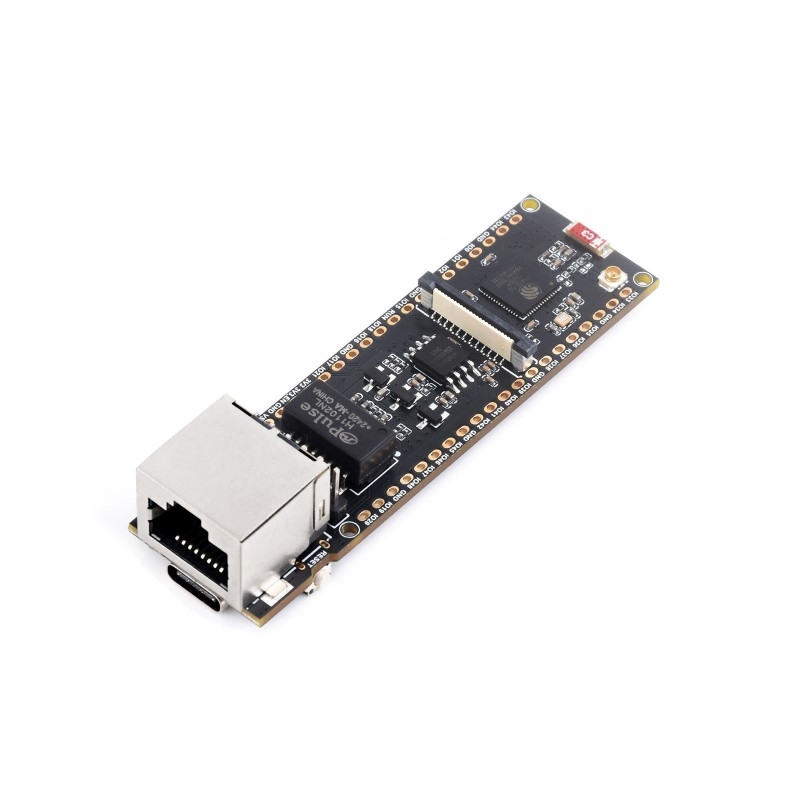
\includegraphics[width=0.55\textwidth]{assets/HW/Waveshare-ESP-S3.jpg}
        \caption{Picture of the Waveshare ESP32-S3 ETH Development Board\cite{noauthor_esp32-s3_nodate}.}
        \label{fig:bridge-node}
    \end{figure}
    
    The bridge node is powered over the USB-C connector. The W5500 is connected to the
    ESP32-S3 over SPI.

    \begin{figure}[H]
        \centering
        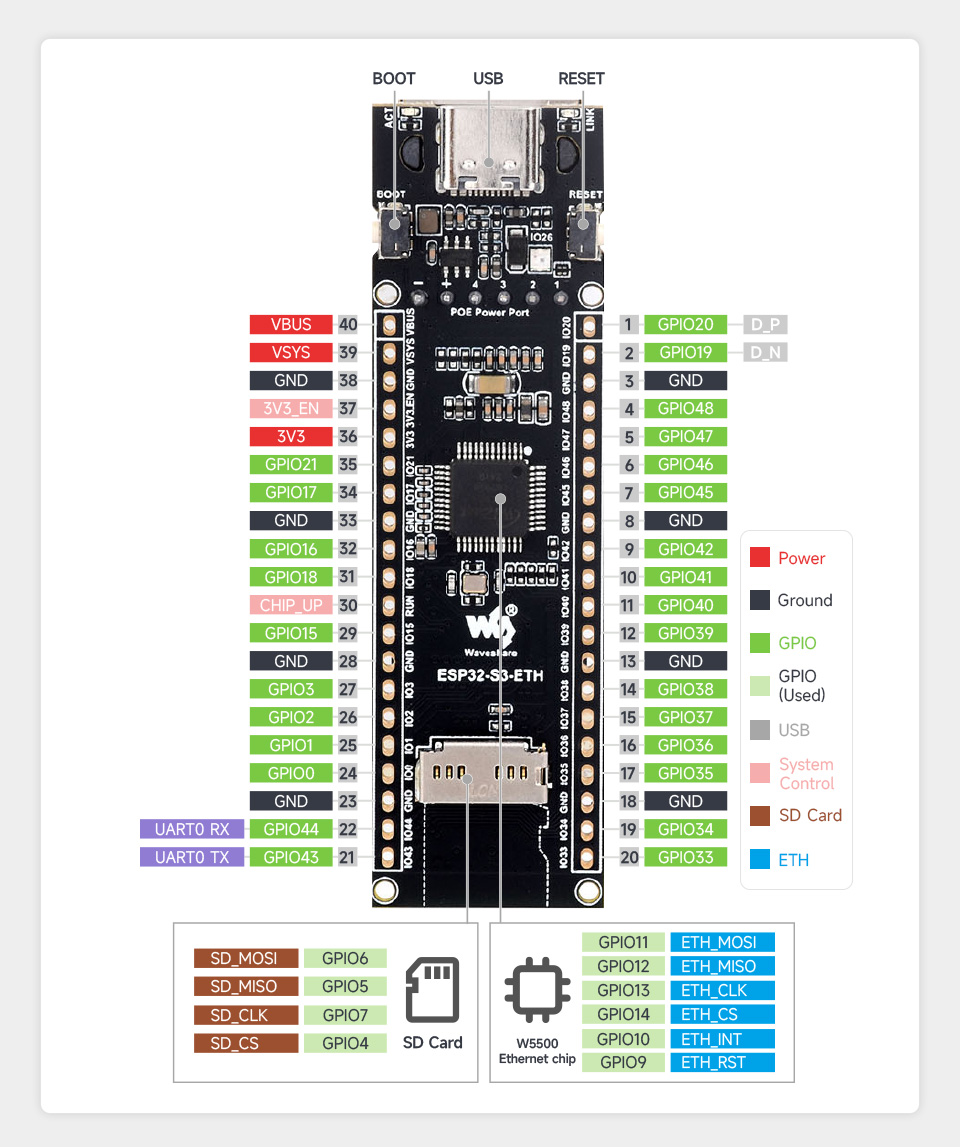
\includegraphics[width=0.6\textwidth]{assets/HW/ESP32-S3-ETH-details-15.jpg}
        \caption{Pinning of the Waveshare ESP32-S3 ETH Development Board\cite{noauthor_esp32-s3_nodate}.}
        \label{fig:bridge-node-detail}
    \end{figure}


%DESCRIBE CODE OF BRIDGE NODE